\documentclass[a4paper,10pt]{article}
\usepackage[a4paper, hmargin={1.5cm,1.5cm}, vmargin={1.5cm,1.5cm}]{geometry}
\usepackage{amsmath}
\usepackage{amssymb}
\usepackage{amsthm}
\usepackage{amsfonts}
\usepackage{color}
\usepackage{graphicx}
\usepackage{listings}

\begin{document}
	
	\textbf{REPORT : Afifah Maya Iknaningrum (1715011053)} \\ \\
	\underline{\textbf{Problem :}}\\
	Make a program code of Euler Method and classical Runge-Kutta for
	\[\begin{cases}
	y' = 5(2-y)y \ \ (0 \leq t \leq 1)\\
	y(0) = 0.04
	\end{cases}\]
	with C language and draw a graph to compare the numerical solution and exact solution for $ N =4,8,16,32,64,128 $ and $ h=1/N $. The exact solution is
	\[ y(t) = \dfrac{2}{1+49e^{-10t}} \]
	\underline{\textbf{C Code :}} \\
	\lstset{
		language=C,                % choose the language of the code
		numbers=left,                   % where to put the line-numbers
		stepnumber=1,                   % the step between two line-numbers.        
		numbersep=5pt,                  % how far the line-numbers are from the code
		backgroundcolor=\color{white},  % choose the background color. You must add \usepackage{color}
		showspaces=false,               % show spaces adding particular underscores
		showstringspaces=false,         % underline spaces within strings
		showtabs=false,                 % show tabs within strings adding particular underscores
		tabsize=2,                      % sets default tabsize to 2 spaces
		captionpos=b,                   % sets the caption-position to bottom
		breaklines=true,                % sets automatic line breaking
		breakatwhitespace=true,         % sets if automatic breaks should only happen at whitespace
		title=\lstname,                 % show the filename of files included with \lstinputlisting;
	}
	
	\lstinputlisting{Euler.c}
	
	\underline{\textbf{GNUPLOT : }}
	\begin{figure}[h!]
		\centering
		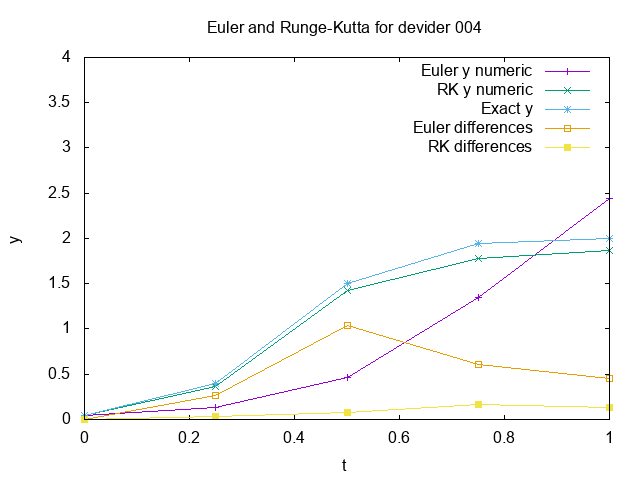
\includegraphics[width=0.7\linewidth]{plot004}
		\caption{}
		\label{fig:plot004}
	\end{figure}
	\begin{figure}[h!]
		\centering
		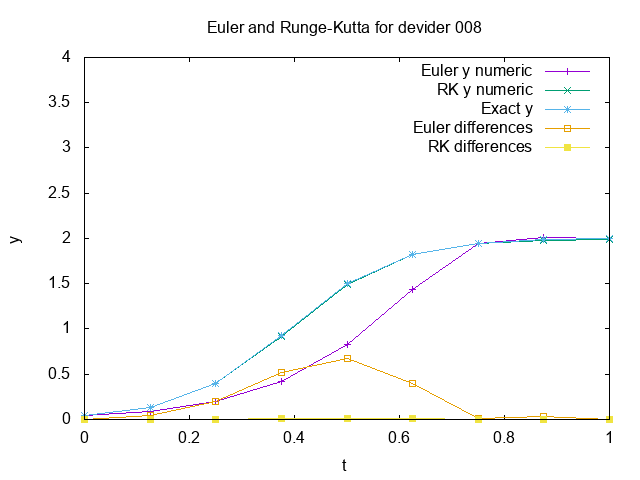
\includegraphics[width=0.7\linewidth]{plot008}
		\caption{}
		\label{fig:plot008}
	\end{figure}
	\begin{figure}[h!]
		\centering
		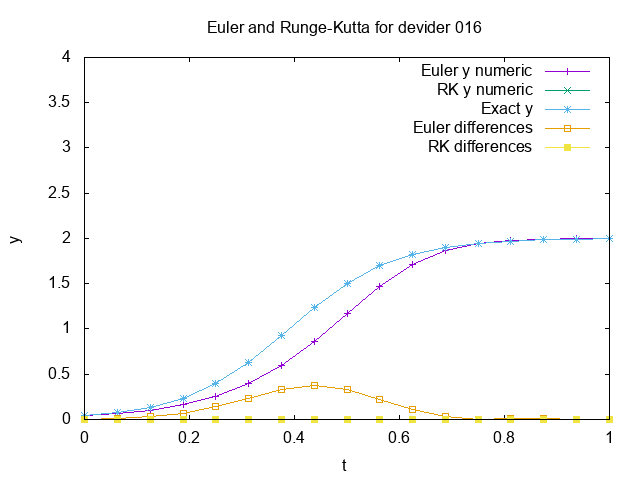
\includegraphics[width=0.7\linewidth]{plot016}
		\caption{}
		\label{fig:plot016}
	\end{figure}
	\begin{figure}[h!]
		\centering
		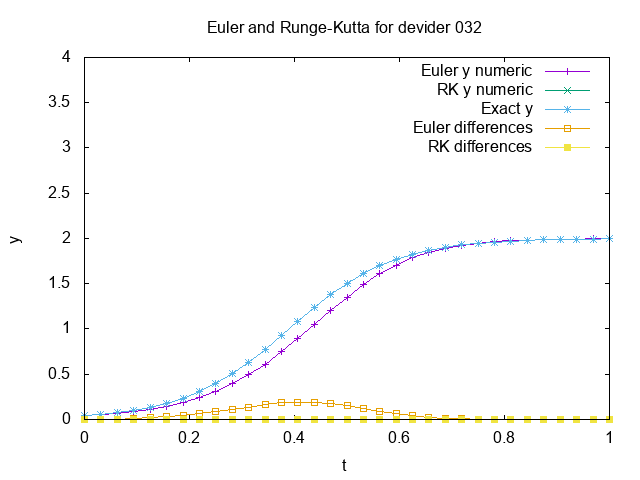
\includegraphics[width=0.7\linewidth]{plot032}
		\caption{}
		\label{fig:plot032}
	\end{figure}
	\begin{figure}[h!]
		\centering
		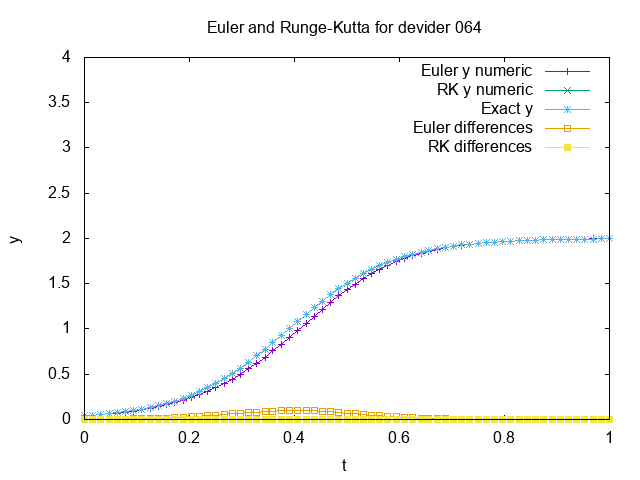
\includegraphics[width=0.7\linewidth]{plot064}
		\caption{}
		\label{fig:plot064}
	\end{figure}
	\begin{figure}[h!]
		\centering
		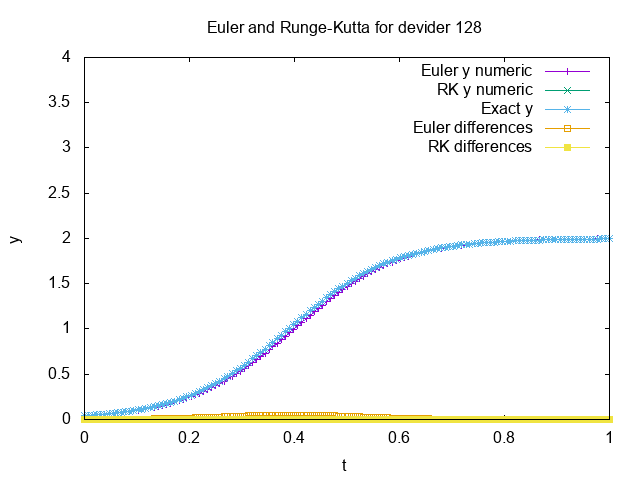
\includegraphics[width=0.7\linewidth]{plot128}
		\caption{}
		\label{fig:plot128}
	\end{figure}
	
\end{document}